\chapter{System Design and Requirements}
\label{chapter:design}

\newenvironment{design}
{\quote\itshape}
{\endquote}

\begin{design}
    This chapter explores the primary architecture that supports the application, outlining its core components and 
    interactions. Also, it covers the basic use cases, along with a comprehensive examination of both 
    functional and non-functional requirements essential for the system's optimal performance.
\end{design}

\section{Basic Use Cases}
The diagram \ref{fig:use-cases} outlines the primary use cases of the application, structured around the user 
interaction flow.

\begin{figure}[h]
    \centering 
    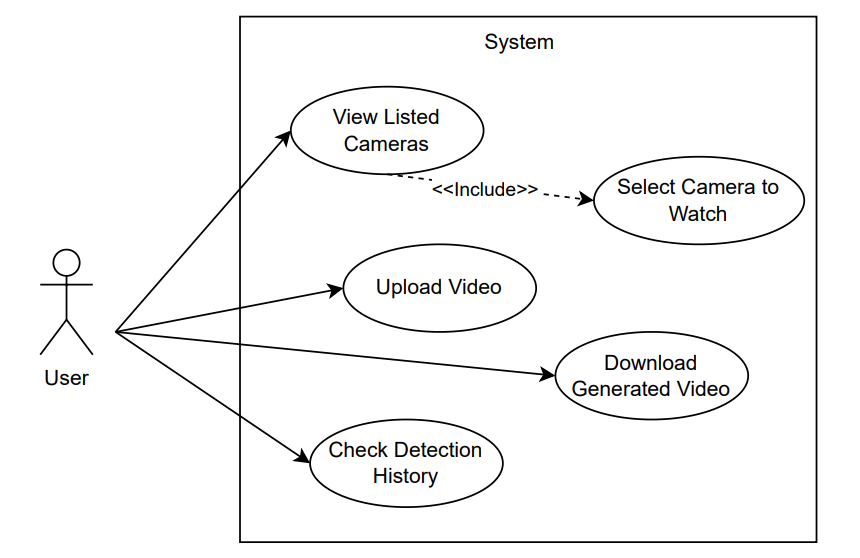
\includegraphics[width=0.6\textwidth]{figs/use-cases3.png} 
    \caption{System Basic Use Cases}
    \label{fig:use-cases}
\end{figure}

At the initial stage, users are presented with a list of all cameras that are registered under their account. 

This list not only displays each camera but also includes information such as the camera's location and current operational
status. Users can conveniently view real-time video streams from these cameras through the application's interface.

Upon viewing the list, users can select any camera to access a more detailed monitoring view. This action 
redirects to a specific page where the video feed from the chosen camera is displayed. This page works 
as the hub for real-time video analysis. While monitoring the video feed, the application actively scans the stream 
for the presence of weapons. If the detection model identifies a weapon within the video, the system generates an alert.

In addition the application supports the upload of pre-recorded videos. Users can upload video files to the platform, which 
are then analyzed by the same detection algorithms used for live streaming.

After uploading a video for analysis, the system processes and annotates the footage with bounding boxes to 
highlight detected weapons. Once the analysis is complete, users have the option to download the annotated video.

Users can also access a comprehensive log of all detection events. This historical data includes detailed information 
about each detection instance, such as the date, time, and frame, enabling users to review past incidents and 
analyze detection patterns over time.

\section{Functional Requirements}
The main goal is to design and implement a real-time weapon detection system capable of 
analyzing surveillance footage and triggering immediate alerts. A prototype showcasing this functionality was developed. 
However, during testing and demonstrations, limitations became evident. Sometimes video streams wouldn't load consistently, 
and alerts were slow to generate. Feedback from security personnel emphasized the need for a more user-friendly 
interface, allowing for quick navigation between cameras and detailed information about detections.

These critical insights guided the development of the core functionalities outlined below:

\begin{enumerate}
    \item Video Stream Handling
    \begin{itemize}
    \item The system shall accept video feeds from various sources, continuously monitoring the video streams 
    and analyze frames for weapon detection;
    \end{itemize}
    \item Detection and Alert Mechanism
    \begin{itemize}
    \item The system shall employ an advanced image recognition algorithm to detect weapons with at least 95\% accuracy;
    \item The system shall generate real-time alerts upon detecting a weapon;
    \item The system shall classify and log each detection event, including time, location, and type of weapon detected;
    \end{itemize}
    \item User Interface
    \begin{itemize}
    \item The system shall offer a user-friendly interface with a dashboard displaying all active video streams;
    \item The interface shall allow operators to navigate easily between different video feeds and alert logs;
    \item The interface shall provide real-time notifications and display detailed information about each detection event;
    \end{itemize}
    \item Data Management
    \begin{itemize}
    \item The system shall store video footage and detection logs securely;
    \item The system shall allow authorized personnel to access and retrieve stored video footage and 
    logs for review and analysis;
    \end{itemize}
    \item Access Control and Security
    \begin{itemize}
    \item The system shall implement user authentication mechanisms to verify the identity of users;
    \end{itemize}
    \item Reliability and Availability
    \begin{itemize}
    \item The system shall include failover protocols to switch to backup systems in case of hardware or software failures;
    \item The system shall monitor its own health and alert administrators to potential issues or failures;
    \end{itemize}
    \item Performance Monitoring
    \begin{itemize}
    \item The system shall continuously monitor its performance, including latency and throughput metrics;
    \item The system shall log performance data and provide administrators with tools to analyze and 
    optimize system performance;
    \item The system shall generate reports on detection accuracy and system performance for regular review.
    \end{itemize}
    \end{enumerate}

\section{High Level Architecture}
Figure \ref{fig:architecture-proposal} illustrates the architecture for the proposed system to 
automatically detect weapons. 

\begin{figure}[ht]
    \centering 
    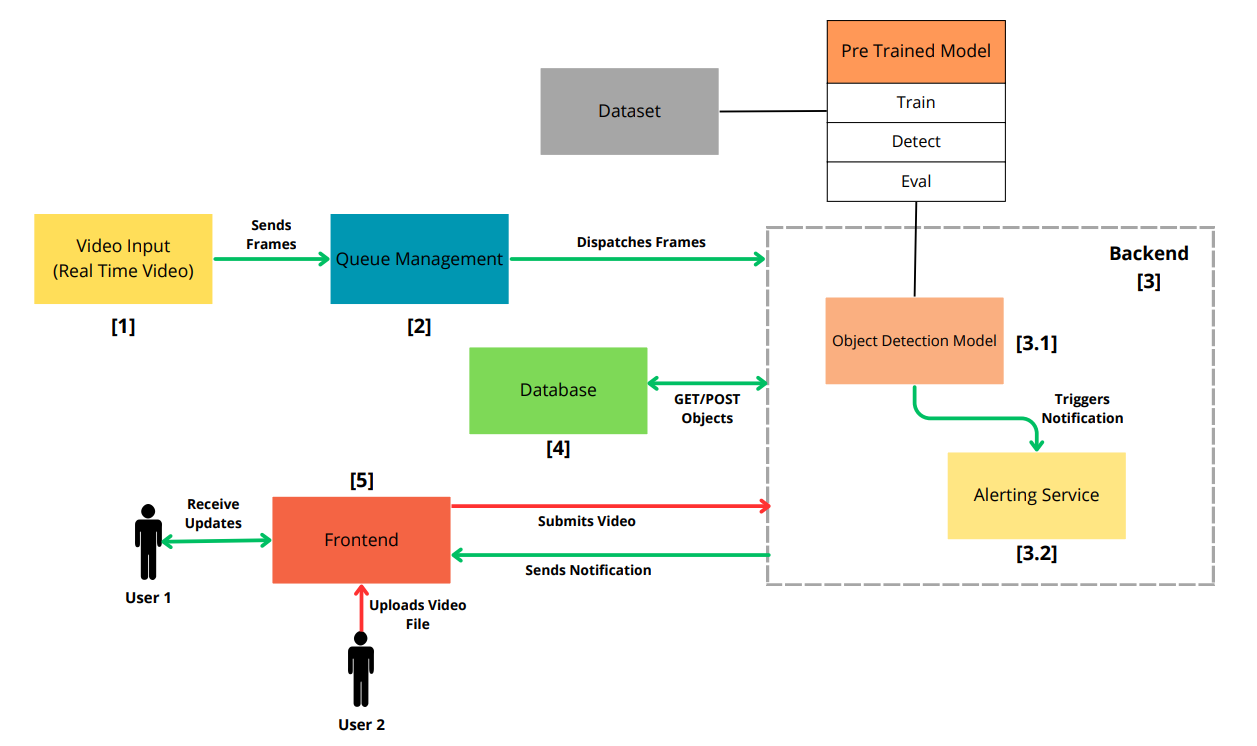
\includegraphics[width=0.95\textwidth]{figs/high-level.png} 
    \caption{High Level Architecture Proposal}
    \label{fig:architecture-proposal}
\end{figure}

% The Video Input (Real-Time Video) [1] consisting of \ac{cctv} cameras strategically installed across various locations, serves as the primary source of video data. These cameras are engineered to capture and transmit real-time video footage, which is then relayed frame by frame to the system for subsequent processing.

The module Video Input (Real-Time Video) [1] aims to feed the system with real-time video using the various \ac{cctv} 
cameras that are spread across various locations.  The video is presented to the system frame by frame, and analyzed 
in the following modules.

% The Queue Management component [2] plays a key role in regulating the incoming data flow. It is specifically tasked with receiving video frames from the \ac{cctv} cameras and systematically queuing them for processing. This component is crucial for several reasons:
The Queue Management component [2] deals with incoming data from previous module, and redeals with incoming data 
from previous module, and regulates the sequence flow. This is a management task, from the balance of received frames 
and sending to futher analysis. Therefore, the following items enumerates the tasks that are associated to this module:

\begin{itemize}
    \item Load Balancing: manages the influx of video frames, particularly crucial during periods of high input. Without this, the backend could become overwhelmed, potentially leading to delays or processing failures;
    \item Prioritization: allows the prioritization of video frames or streams, especially those from high-risk areas;
    \item Scalability: enables efficient scaling without necessitating significant modifications to the backend processing infrastructure.
\end{itemize}

The backend [3] serves as the system's "central processing unit". It is composed by a set of submodules:
\begin{itemize}
    \item Object Detection Model [3.1]: designed to identify objects of interest, primarily focusing on potentially dangerous items like firearms and knives. It operates with a pre-trained model that was trained on a dataset, which has been finely tuned to pinpoint threats with precision.
    \item Alerting Service [3.2]: upon detection of a hazardous object, it promptly generates notifications/alerts. These alerts are then swiftly relayed to the frontend, thereby enabling law enforcement officials to receive real-time updates and respond accordingly.
\end{itemize}

The database [4] stores the critical data gererated by the system, like que video metadata, logs of detected objects, 
model-related data, and other information that supports the system.

Finally, the Frontend [5] enables the interface between system and end users (such as law enforcement officers). Tasks like the uploading of video files for analysis can be performed throw  this interface. Moreover, it serves as a dynamic platform for receiving timely updates and alerts regarding any detected objects, thereby streamlining the communication process and enhancing the efficiency of law enforcement responses.

\section{Non-Functional Requirements}
This section outlines the non-functional requirements essential for the system's successful implementation and operation.
Non-functional requirements define the system's operational attributes, which are crucial to ensuring the system's 
efficiency and effectiveness in real-world scenarios. 

The non-functional requirements can be categorized as follows:
\begin{enumerate}
    \item Performance
    \begin{itemize}
        \item Latency: the system must process video frames with minimal delay to ensure real-time detection;
        \item Throughput: the system should handle multiple video streams simultaneously without significant 
        performance degradation;
        \item Accuracy: high detection accuracy is essential to minimize false positives and false negatives;
    \end{itemize}
    \item Reliability and Availability
    \begin{itemize}
        \item Uptime: the system must maintain high availability, ensuring
        continuous surveillance and monitoring without interruptions;
        \item Fault Tolerance: the system should be resilient to hardware and software failures;
        %\item Accuracy: High detection accuracy is essential to minimize false positives and false negatives. 
    \end{itemize}
    \item Security
    \begin{itemize}
        \item Data Protection: the system must ensure the confidentiality and integrity of video footage. This includes 
        secure data transmission and storage using encryption methods to prevent unauthorized access;
        \item Access Control: strict access control mechanisms should be implemented to restrict system usage to 
        authorized personnel only;
    \end{itemize}
    \item Usability
    \begin{itemize}
        \item User Interface: the system must provide an intuitive and user-friendly interface for 
        operators. This
        includes clear visual indicators for detected threats and straightforward navigation to view 
        video feeds and alerts.
    \end{itemize}
  \end{enumerate}

  \begin{figure}[ht]
    \centering 
    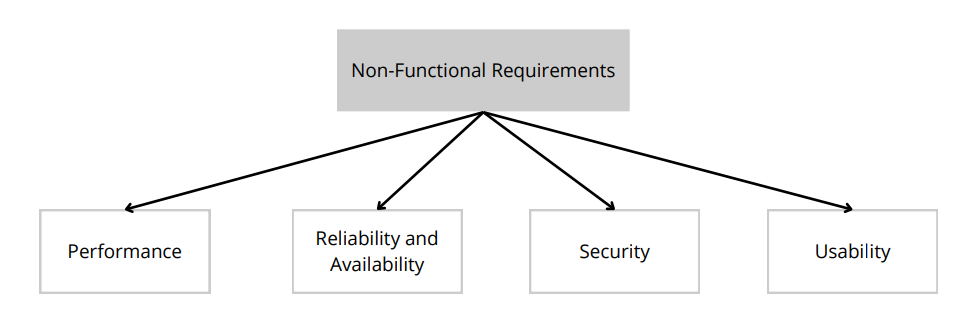
\includegraphics[width=0.65\textwidth]{figs/requirements.png} 
    \caption{Non-Functional Requirements}
    \label{fig:non-requirements}
\end{figure}